% Enable warnings about problematic code
\RequirePackage[l2tabu, orthodox]{nag}

\documentclass{WeSTassignment}

% The lecture title, e.g. "Web Information Retrieval".
\lecture{Introduction to Web Science}
% The names of the lecturer and the instructor(s)
\author{
  Prof. Dr.~Steffen~Staab\\{\normalsize\mailto{staab@uni-koblenz.de}} \and
  Ren{\'e}~Pickhardt\\{\normalsize\mailto{rpickhardt@uni-koblenz.de}} \and
   Korok~Sengupta\\{\normalsize\mailto{koroksengupta@uni-koblenz.de}} \and 
   Olga~Zagovora\\{\normalsize\mailto{zagovora@uni-koblenz.de}}
}
% Assignment number.
\assignmentnumber{10}
% Institute of lecture.
\institute{%
  Institute of Web Science and Technologies\\%
  Department of Computer Science\\%
  University of Koblenz-Landau%
}
% Date until students should submit their solutions.
\datesubmission{January 25, 2016, 10:00 a.m.}
% Date on which the assignments will be discussed in the tutorial.
\datetutorial{January 27, 2016, 12:00 p.m.}

% Set langauge of text.
\setdefaultlanguage[
  variant = american, % Use American instead of Britsh English.
]{english}

% Specify bib file location.
\addbibresource{bibliography.bib}

% For left aligned centerd boxes
% see http://tex.stackexchange.com/a/25591/75225
\usepackage{varwidth}

% ==============================================================================
% Document

\begin{document}

\maketitle


For all the assignment questions that require you to write code, \textbf{make sure to include the code in the answer sheet, along with a separate python file. Where screen shots are required, please add them in the answers directly and not as separate files.}\\ \\ 

%Please mention your team Names here: 
Team Name: hotel

Andrea Mildes - mildes@uni-koblenz.de

Sebastian Blei - sblei@uni-koblenz.de

Johannes Kirchner - jkirchner@uni-koblenz.de

Abdul Afghan - abdul.afghan@outlook.de


\section{Modeling Twitter data (10 points)}

In the meme paper\footnote{\url{http://www.nature.com/articles/srep00335}} by Weng et al., in Figure 2\footnote{Slide 27, Lecture Meme spreading on the Web} you find a plot, comparing the system entropy with the average user entropy. Your task is to reproduce the plot and corresponding calculations.
\begin{enumerate}
\item We provide you with the file 'onlyhashtag.data’, containing a collection
of hashtags from tweets. Use this data to reproduce the plot from the paper.
Once you have the values for average user entropy and system entropy calculated
per day create a scatter plot to display the values.
\item Interpret the scatter plot and compare it with the authors interpretation from the
graph 
%produced on the previous step and 
showed in the paper. Will the interpretations be compatible to each other or will they contradict each other? Do not write more than 5 sentences.
\end{enumerate}





\subsection{Hints}
\begin{enumerate}
\item Use formulas from the lecture to calculate the entropy for one user and the system entropy.
\item Do not forget to give proper names of plot axes.
\end{enumerate}


%-------------------------------------------------------------------------------

%-------------------------------------------------------------------------------

\section{Measuring inequality (10 points)}

We provide you with a sample implementation of the Chinese Restaurant Process\footnote{File ``chinese\_restaurant.py"; Additional information can be found here: \url{https://en.wikipedia.org/wiki/Chinese_restaurant_process}}.

Assume there is a restaurant with an infinite number of tables. 
When a new customer enters a restaurant he chooses an occupied table or the next empty table with some probabilities.


According to the process first customer always sits at the first table. 
Probability of the next customer to sit down at an occupied table $i$ equals 
 ratio of guests sitting at the table ($c_i/n$), where $n$ is the number of guests in the restaurant and $c_i$ is the number of guests sitting at table $i$.\\
 Probability of customer to choose an empty table equals :  $1- \sum_{i=1}^{S}{p_i}$, where $S$ is the number of occupied tables and ${p_i}$ = $c_i/n$.
 
Provided script simulates the process and returns number of people sitting at each table. We will study restaurants for 1000 customers.
Now you should modify the code and evaluate how unequal were the customers' choices of tables.   

%In this exercise,
%you should use it to simulate the growth of a network via the following process:
%\begin{itemize}
%\item A customer X sitting at a table Y, represents an edge from node X to node Y .
%\item With X tables occupied, a new customer taking a new table, will take place at table X + 1.
%\end{itemize} 

% In the lecture `Herding Behavior' we discussed paper\footnote{`Experimental Study of Inequality and Unpredictability in an Artificial Cultural Market.', can be accessed from  \url{https://www.princeton.edu/~mjs3/salganik_dodds_watts06_full.pdf} } by Salganik et al. The authors used the Gini-coefficient to measure the inequality and in the lecture you have see how this coefficient stabilizes over time.

%Simulate a network with the Chinese Restaurant process and 
Calculate the Gini-
coefficient measuring the inequality between the tables,
until the coefficient stabilizes. Do five different runs and plot your results in a similar way that plots in the lecture slides are done, cf. Slide 32 and Slide 33.

\textbf{Code:}
\lstinputlisting{chinese_restaurant.py}
\textbf{Output:}\\
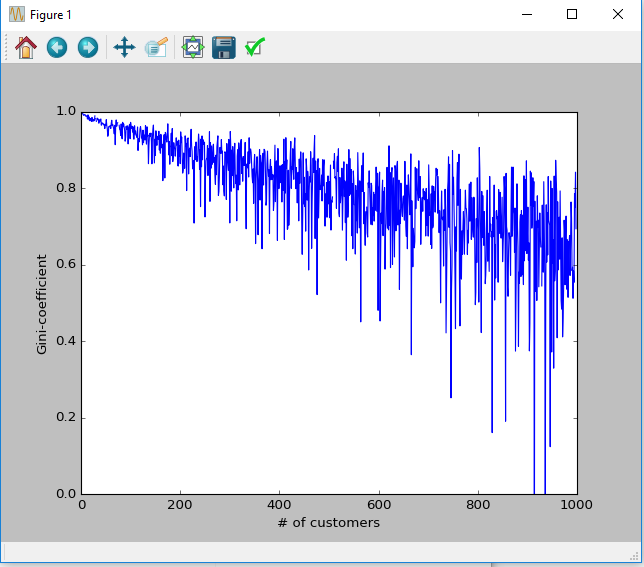
\includegraphics[width=400px]{1stPlot}\\
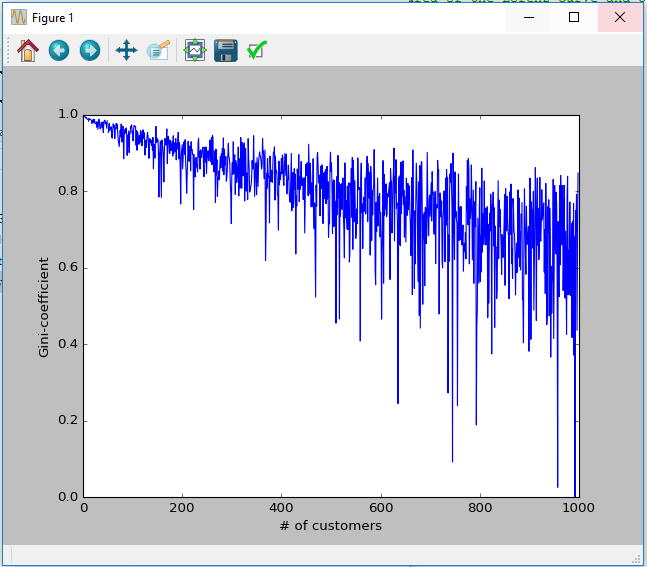
\includegraphics[width=400px]{2ndPlot}\\
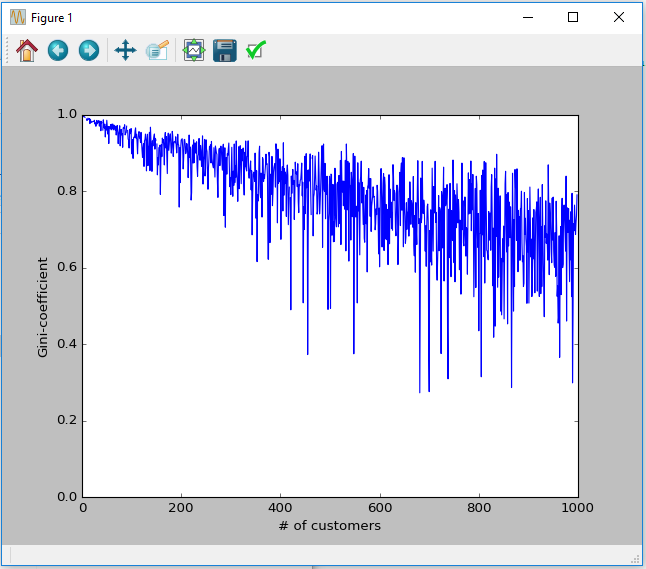
\includegraphics[width=400px]{3rdPlot}\\
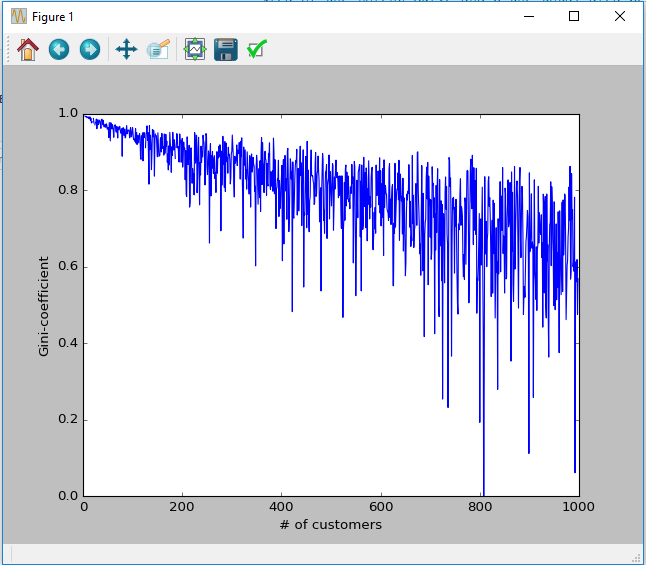
\includegraphics[width=400px]{4thPlot}\\
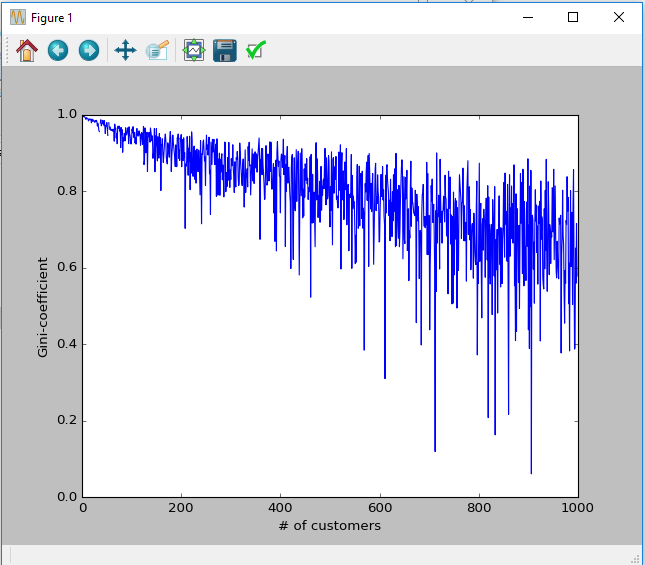
\includegraphics[width=400px]{5thPlot}\\


%-------------------------------------------------------------------------------

%-------------------------------------------------------------------------------

\section{Herding (10 points)}
Let us consider the altitude of Koblenz to be 74 m above sea level. You are asked to figure out the height of the Ehrenbreitstein Fortress and the Fernmeldeturm Koblenz without googling.\\
The exercise is split in two parts:\\ \\
\underline{Part 1 : The Secret}\\
In \textit{complete secrecy}, each member of the team will write down their estimated height of the Ehrenbreitstein Fortress without any form of discussion. Please keep in mind that you need to have reasons for your assumption. Once you are done, then openly discuss in the group and present you values in a tabulated format with the reasons each one assumed to arrive at that value. 

\underline{Part II : The Discussion}\\
Discuss amongst yourself with valid reasoning  what could be the height of the Fernmeldeturm Koblenz. Only after discussing, each member of the group is asked to arrive at a value and present this value in a tabulated format as was done in Part I. \\ \\
Calculate the Mean, Standard Deviation and Variance of your noted results for both the cases and explain briefly what you infer from it. 

\textbf{Note:} This exercise is for you to understand the concepts of herding and not to get the perfect height by googling information. There is in fact no point associated with the height but with the complete reasoning that you provide for your answers. 



\emph{Solution:}

Part 1: \\

\begin{tabular}{l|c}
  Sebastian: & 189\\
  Johannes: & 274\\
  Andrea: & 249
 \end{tabular}

Sebastian: 115 + 74; Sebastian recalled his ride with the ropeway to Ehrenbreitstein and estimated the height by taking the duration and speed of the ride into consideration. \\\\
Johannes: 200 + 74; Johannes estimated the height of Ehrenbreitstein by knowing that most reflector posts have a distance of 50 meters to each other. He than stacked this distance between the posts vertically in his mind and thought that 4 times that distance could be as high as the Fortress, which equals 200 meters. \\\\
Andrea: 175 + 74; Andrea remembered the view from the fortress down to Koblenz and estimated based on the view. 

Mean: $(189 + 274 + 249) / 3 = 237,333$ \\
Variance: $1/2 * ((189 - 237,333)^2 + (274-237,333)^2 + (249 - 237,333)^2) = 1/2 * (2336,079 + 1344,469 +  136,118889) = 1908,3334445$ \\
Standard Deviation: $sqrt(Variance) = 43,684$


Part 2: \\
To be honest: After the first discussion we were curious how high Ehrenbreitstein is, so we googled it.\\ In the second discussion we all agreed that the Karthause (the district where the Fernmeldeturm is located) is roughly as high as Ehrenbreitstein, which is about 118 meters. However, we couldn't agree on the height of the Fernmeldetum itself, so our numbers differ anyways. 

Mean: $(150 + 160 + 210) / 3 = 173,333 $
Variance: $1/2 * ((150-173,333)^2 + (160-173,333)^2 + (210-173,333)^2) = 1/2 * (544,429 + 177,769 + 1344,469) = 1033,333$//
Standard Deviation: $sqrt(Variance) = 32,146$

As calculated, the variance and standard deviation of part 1 are higher than the variance and deviation of part 2. Most probably this was caused by our discussion, which led to more similar hight-assumptions. For example, all of us agreed that the height of the Karthause is about 120 meters, which would not have been the case without a discussion. 

\begin{tabular}{l|cc}
  Sebastian: & 150 & \\
  Johannes: & 160 & \\
  Andrea: & 210 &
\end{tabular}


\makefooter

\end{document}
